\documentclass[a4paper]{scrartcl}

\usepackage[T1]{fontenc}
\usepackage[a4paper, total={6.5in, 8.5in}]{geometry}

\usepackage{multicol}

\usepackage{minted}

\usepackage{hyperref}
\usepackage{cleveref}

\usepackage{pdfpages}

\title{COL216 Assignment 2\\{\Large Stage 1}}
\date{10 February 2022}
\author{Rishabh Dhiman\\ 2020CS10837}

\renewcommand{\tt}{\mintinline{text}}

\begin{document}
\maketitle

\section{Objective}
Construct an ALU, a register file, a primary memory unit and a data memory unit for a rudimentary ARM processor in VHDL.

\section{Technical Details}
\begin{itemize}
	\item The VHDL code was analyzed and simulated using GHDL 1.0.0.
	\item The waveform viewer used is GTKWave Analyzer v3.3.104.
\end{itemize}

\section{Documentation}
The submission contains four VHDL files defining the various units,
\begin{itemize}
	\item \tt{types.vhdl},
	\item \tt{alu.vhdl},
	\item \tt{reg_file.vhdl}, and
	\item \tt{memory.vhdl}.
\end{itemize}
Along with four testbenches for testing these units
\begin{itemize}
	\item \tt{alu_testbench.vhdl},
	\item \tt{reg_file_testbench.vhdl},
	\item \tt{primary_memory_testbench.vhdl}, and
	\item \tt{data_memory_testbench.vhdl}.
\end{itemize}

Along with the code, an output folder, containing the waveforms on simulating the testbenches, in the form of \tt{.ghw} and \tt{.pdf} files are stored in the output folder.

For units with a clock, actions were performed only at the rising edge of the clock.

\subsection*{\tt{types.vhdl}}
This files defines some custom types for words, half-words and bytes along with an enumerated type for the 16 opcodes. It's taken from Piazza post 163, with minor modifications.

\subsection*{\tt{alu.vhdl}}
It defines the ALU satisfying the specifications given in the problem statement.
The entity declaration of the ALU is given by,
\begin{minted}{vhdl}
entity alu is
	port(
		op1, op2: in word;
		result: out word;
		instr: in optype;
		carry_in: in std_logic;
		carry_out: out std_logic);
end alu;
\end{minted}
where \tt{word} and \tt{optype} data types are defined in \tt{types.vhdl}.

In the case of logical operations, the \tt{carry_out} bit is set to $0$.

\subsection*{\tt{memory.vhdl}}
It defines the primary memory and data memory satisfying the specifications given in the problem statement.

Since the program memory is hardcoded, I decided to initialize it such that the $i$-th position stores the value $i$ for ease of testing.

The entity declaration of the program memory is given by
\begin{minted}{vhdl}
entity program_memory is
	port(
		    addr: in word;
		    data_out: out word);
end program_memory;
\end{minted}

The entity declaration of the data memory is given by,
\begin{minted}{vhdl}
entity data_memory is
	port(
		    addr: in word;
		    write_enable: in std_logic_vector(3 downto 0);
		    clock: in std_logic;
		    data_in: in word;
		    data_out: out word);
end data_memory;
\end{minted}

Note that though the memory has only 64 locations, I chose to make \tt{addr} have word length, which is 32 here, to ensure compatibility with the rest of the processor.

\subsection*{\tt{reg_file.vhdl}}
It defines the register file satisfying the specifications given in the problem statement.
The entity declaration of the register file is given by,
\begin{minted}{vhdl}
entity reg_file is
	port(
	read_addr1, read_addr2, write_addr: in std_logic_vector(3 downto 0);
	data_in: in word;
	write_enable: in std_logic;
	clock: in std_logic;
	data_out1, data_out2: out word);
end reg_file;
\end{minted}
Note that unlike with the memories, the addresses are 4-bits.

\section{Testing Procdure}
The code was analyzed and simulated using GHDL.

You can simulate it yourself using the \tt{makefile} provided on.
\begin{enumerate}
	\item Ensure that Make and GHDL are installed.
	\item Navigate to the \tt{src} directory.
	\item Create a folder called \tt{output} inside the \tt{src} directory (if it doesn't exist already).
	\item In the commandline, run \tt{make} or \tt{make all} to analyze, and then simulate the programs.
	\item \tt{.ghw} waveform files will be created in the output directory. Note that the earlier \tt{.ghw} in the output folder will be overwritten.
	\item You can finally run \tt{make clean} to delete any temporary files created in the process.
\end{enumerate}

There are 4 testbenches,
\begin{multicols}{2}
	\begin{itemize}
		\item \tt{alu_tb},
		\item \tt{reg_file_tb},
		\item \tt{data_memory_tb},
		\item \tt{program_memory_tb}.
	\end{itemize}
\end{multicols}

These testbenches follow the rule that ports of the unit being tested are connected to the signals of the same name in the testbench. For example, \mintinline{vhdl}{signal op1} of the testbench \tt{alu_tb} is connected to the port \tt{op2} of the \tt{alu}.

\subsection*{\tt{alu_tb}}
This tests the ALU by iterating over 3 values of the two operands, \tt{0x7FFF_FFFF}, \tt{0x0000_0000}, and \tt{0x0000_0001}, and all possible opcodes and carry-in bits. Giving a total of $16 \times 2 \times 3 \times 3 = 288$ combination.

\subsection*{\tt{program_memory_tb}}
This testbench simply reads the data from the 64 memory addresses sequentially.

\subsection*{\tt{data_memory_tb}}
The clock period of the testbench is 1\,ns.

This testbench first sequentially goes through all 16 values of the \tt{write_enable} vector from \tt{0000} to \tt{1111}. For each such value of \tt{write_enable}, it iterates through all 64 memory locations and passes the value $256x + i$ to \tt{data_in} of the memory, where $x$ is the current value of \tt{write_enable} when viewed as a binary number.

At the end, it sequentially reads all 64 values stored in the memory.

\subsection*{\tt{reg_file_tb}}
The clock period of the testbench is 1\,ns.

The testbench first writes to the memory. It sequentially writes in the value $i$ to memory location $i$. Simultaneously, it reads out the value from memory locations $i$ and $15 - i$. Note that the memory locations read may be uninitialized.

Then, it reads out values from the memory. For every $16 \times 16$ pairs of the two read addresses, the value from these locations is read out of the memory.

\section{Results}
The output waveform of the testbench results can be viewed in .ghw and .pdf files in the output folder.

The .pdf files don't contain the entire waveform as the total number of pages required would be prohibitively large. However, the .ghw files can be opened in any waveform analyzer like GTKWave to view the output waveform.

The pdf files are also attached at the end of this report.

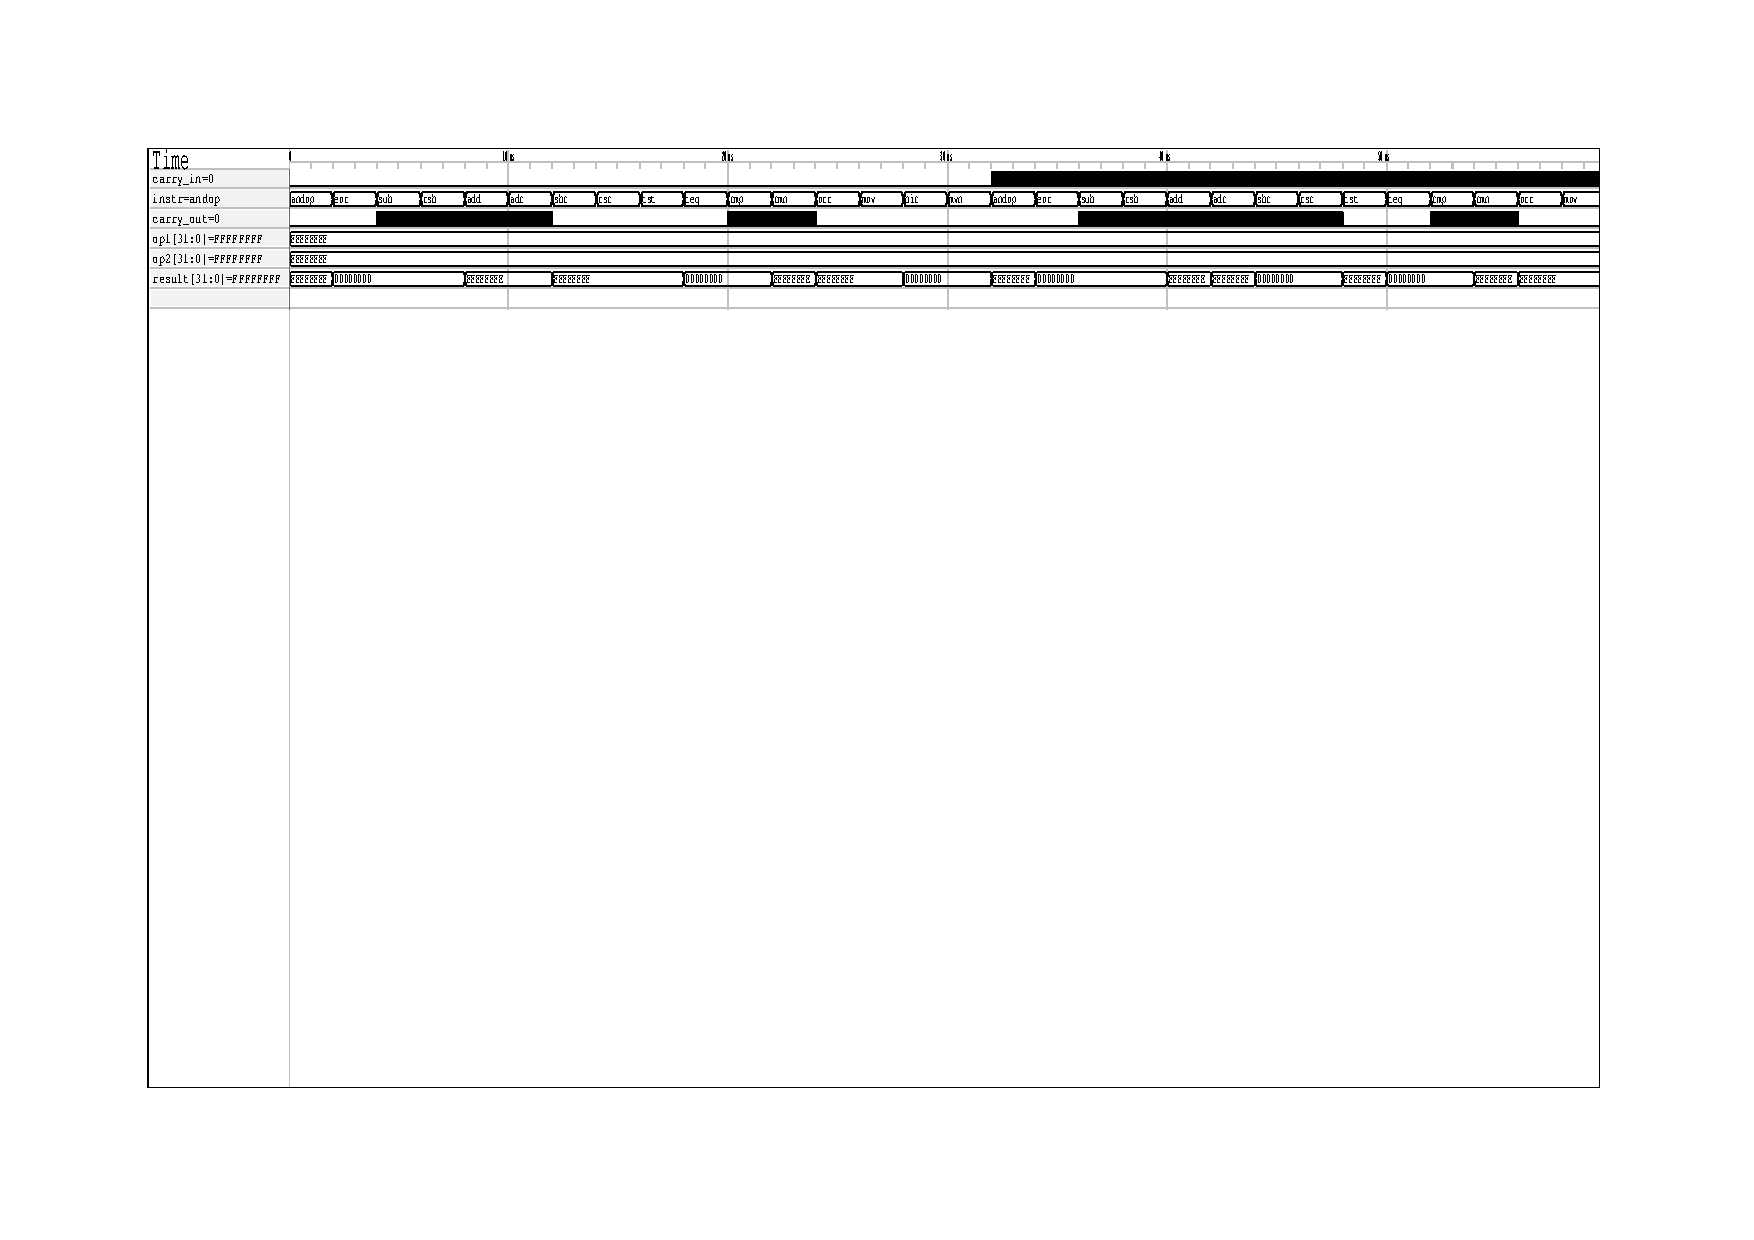
\includepdf[landscape=true, picturecommand*={\put (\LenToUnit{.05\paperwidth},20) {\tt{alu_tb.pdf}};}]{../output/alu_tb.pdf}
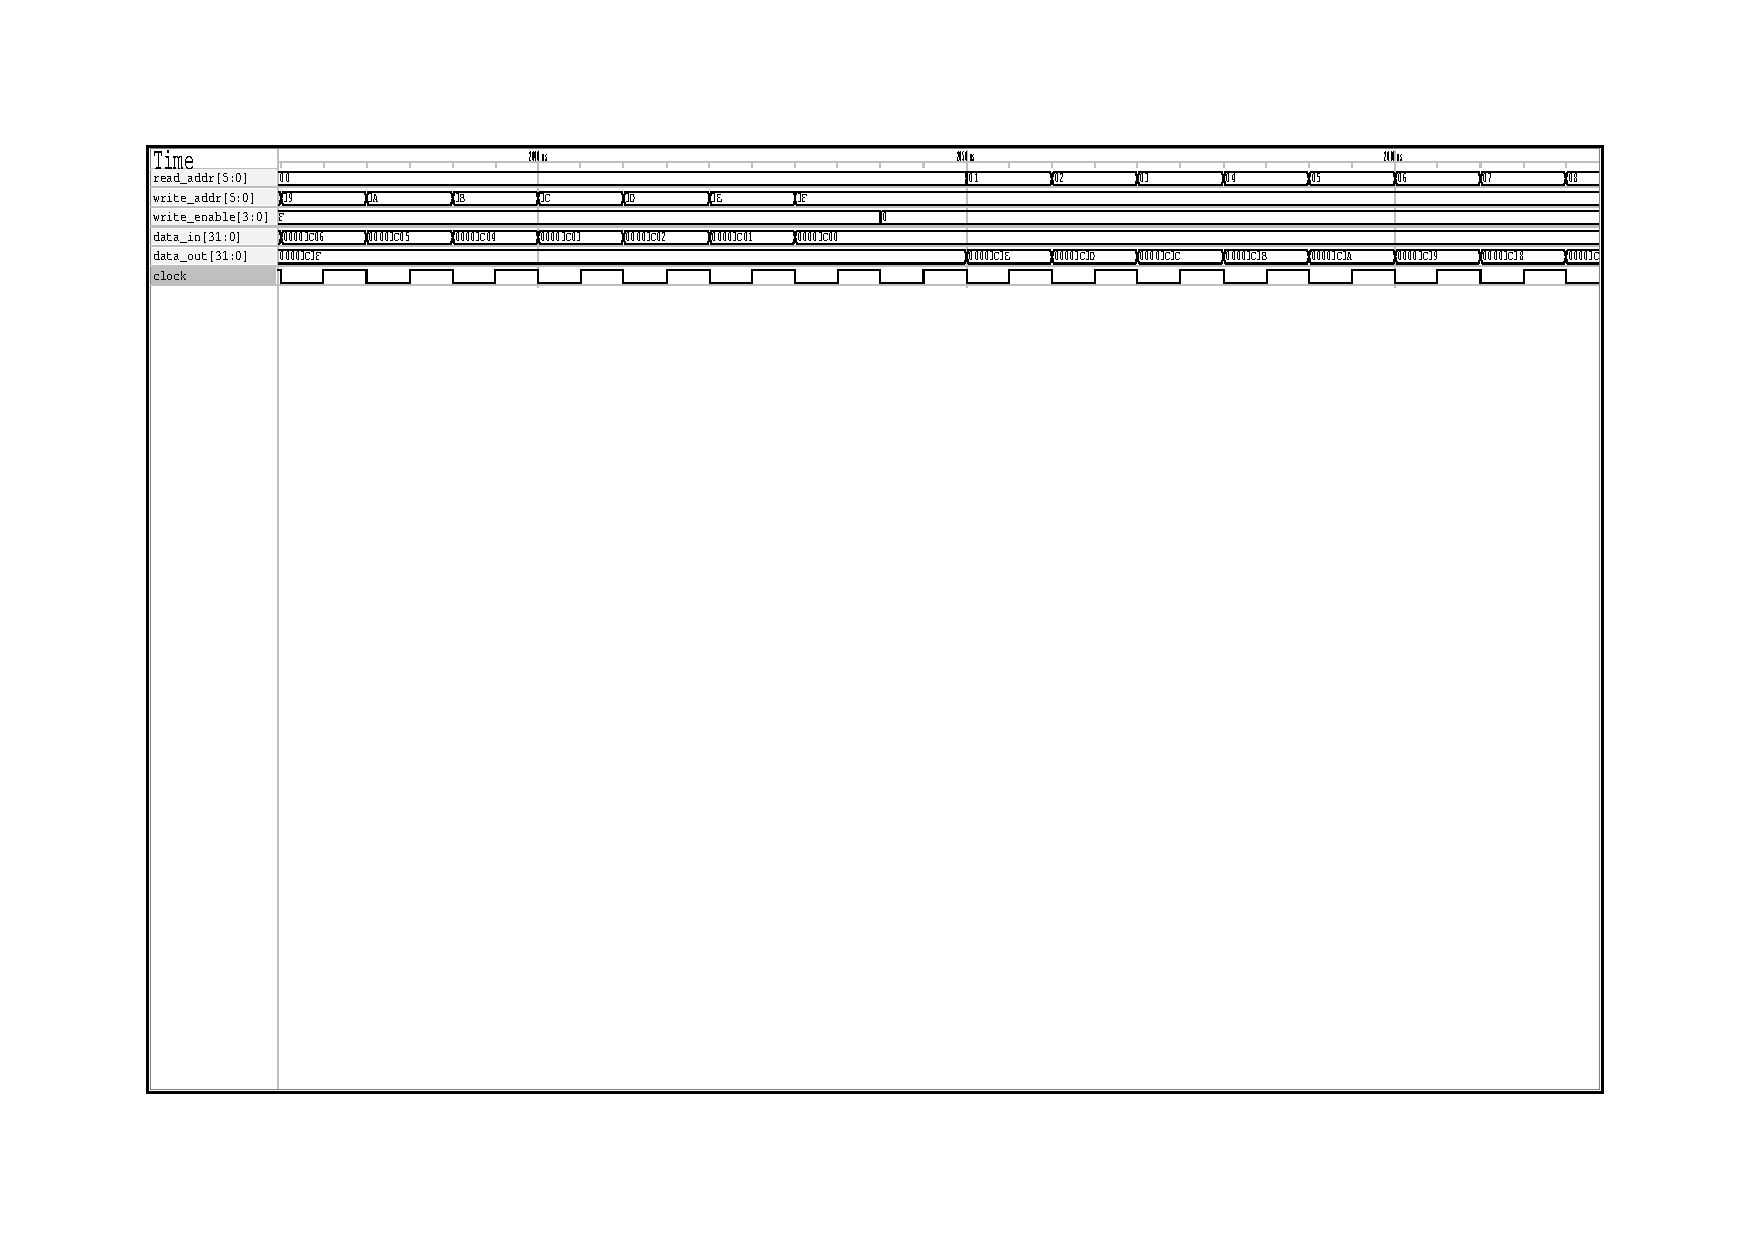
\includepdf[landscape=true, picturecommand*={\put (\LenToUnit{.05\paperwidth},20) {\tt{data_memory_tb.pdf}};}]{../output/data_memory_tb.pdf}
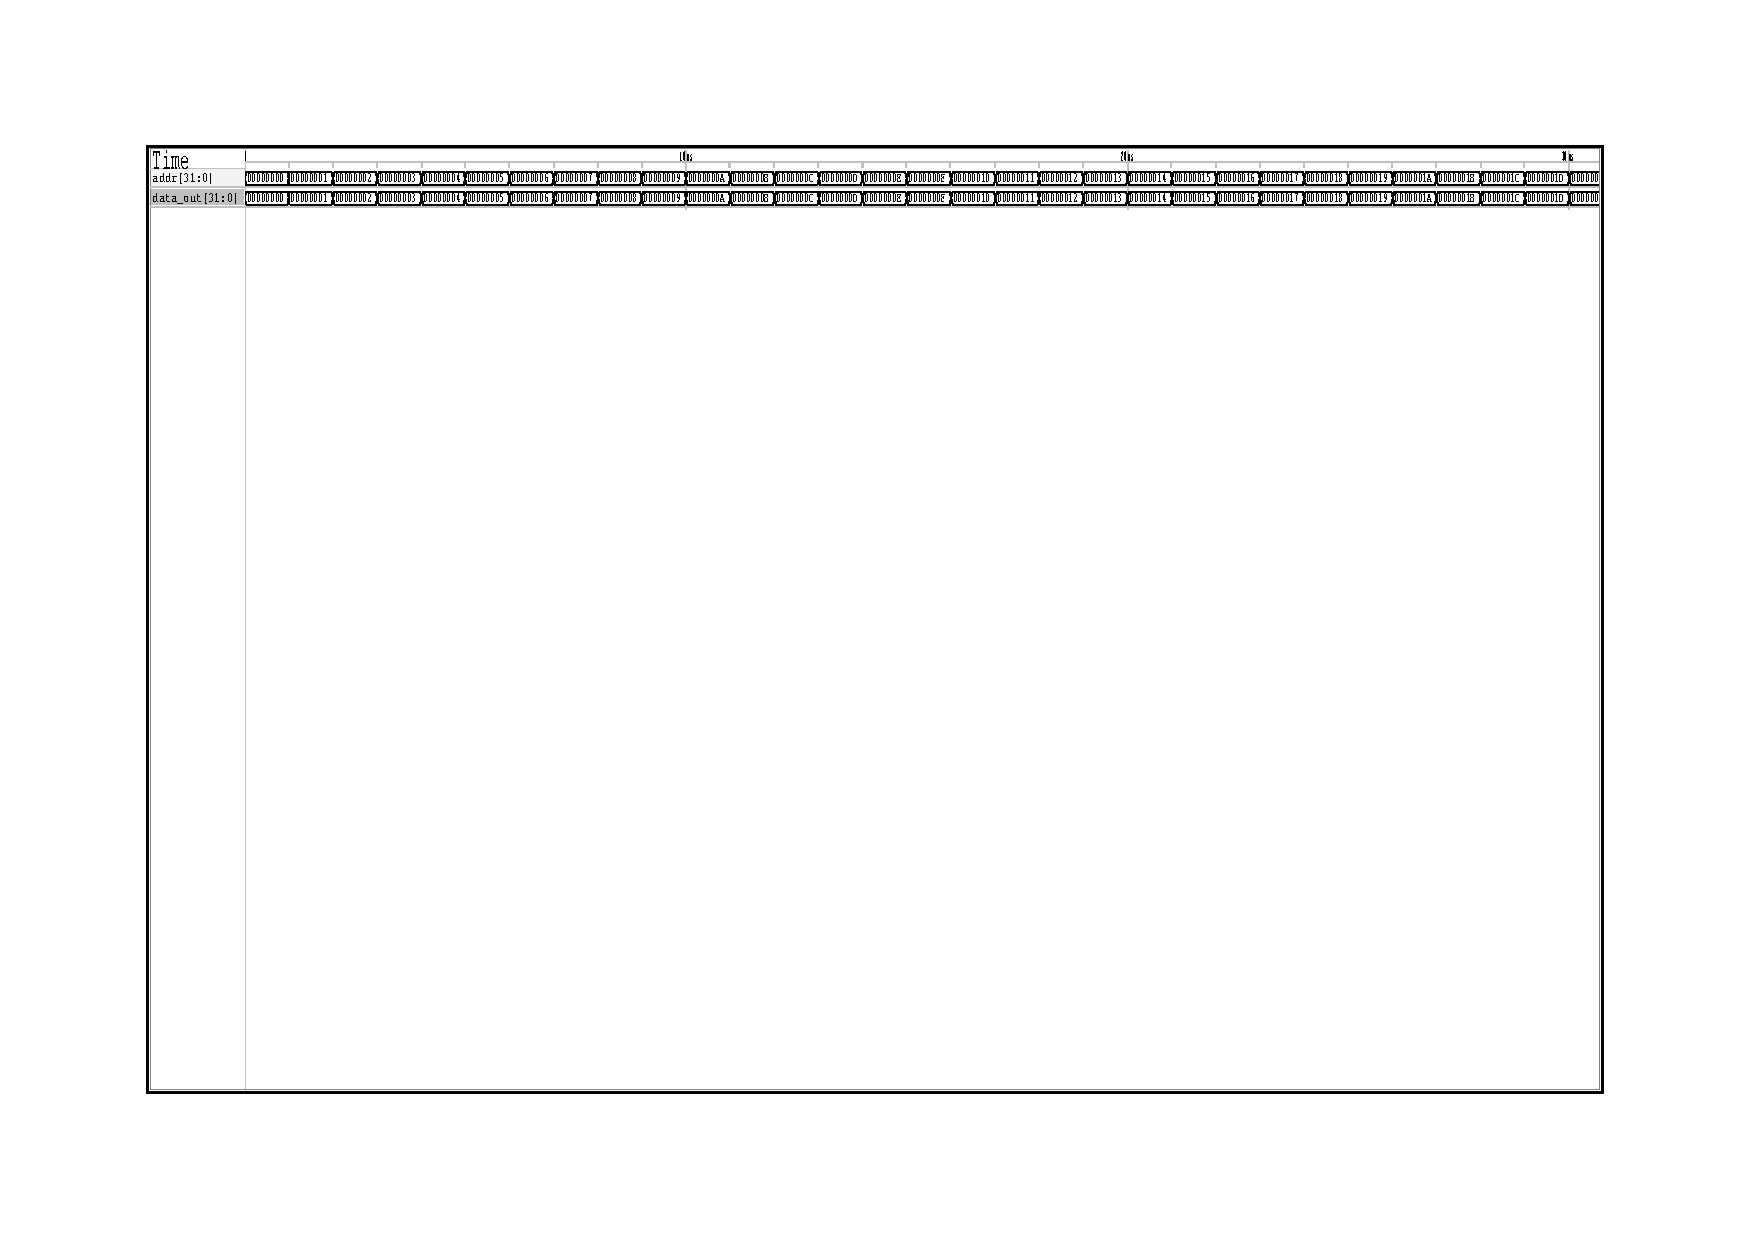
\includepdf[landscape=true, picturecommand*={\put (\LenToUnit{.05\paperwidth},20) {\tt{primary_memory_tb.pdf}};}]{../output/primary_memory_tb.pdf}
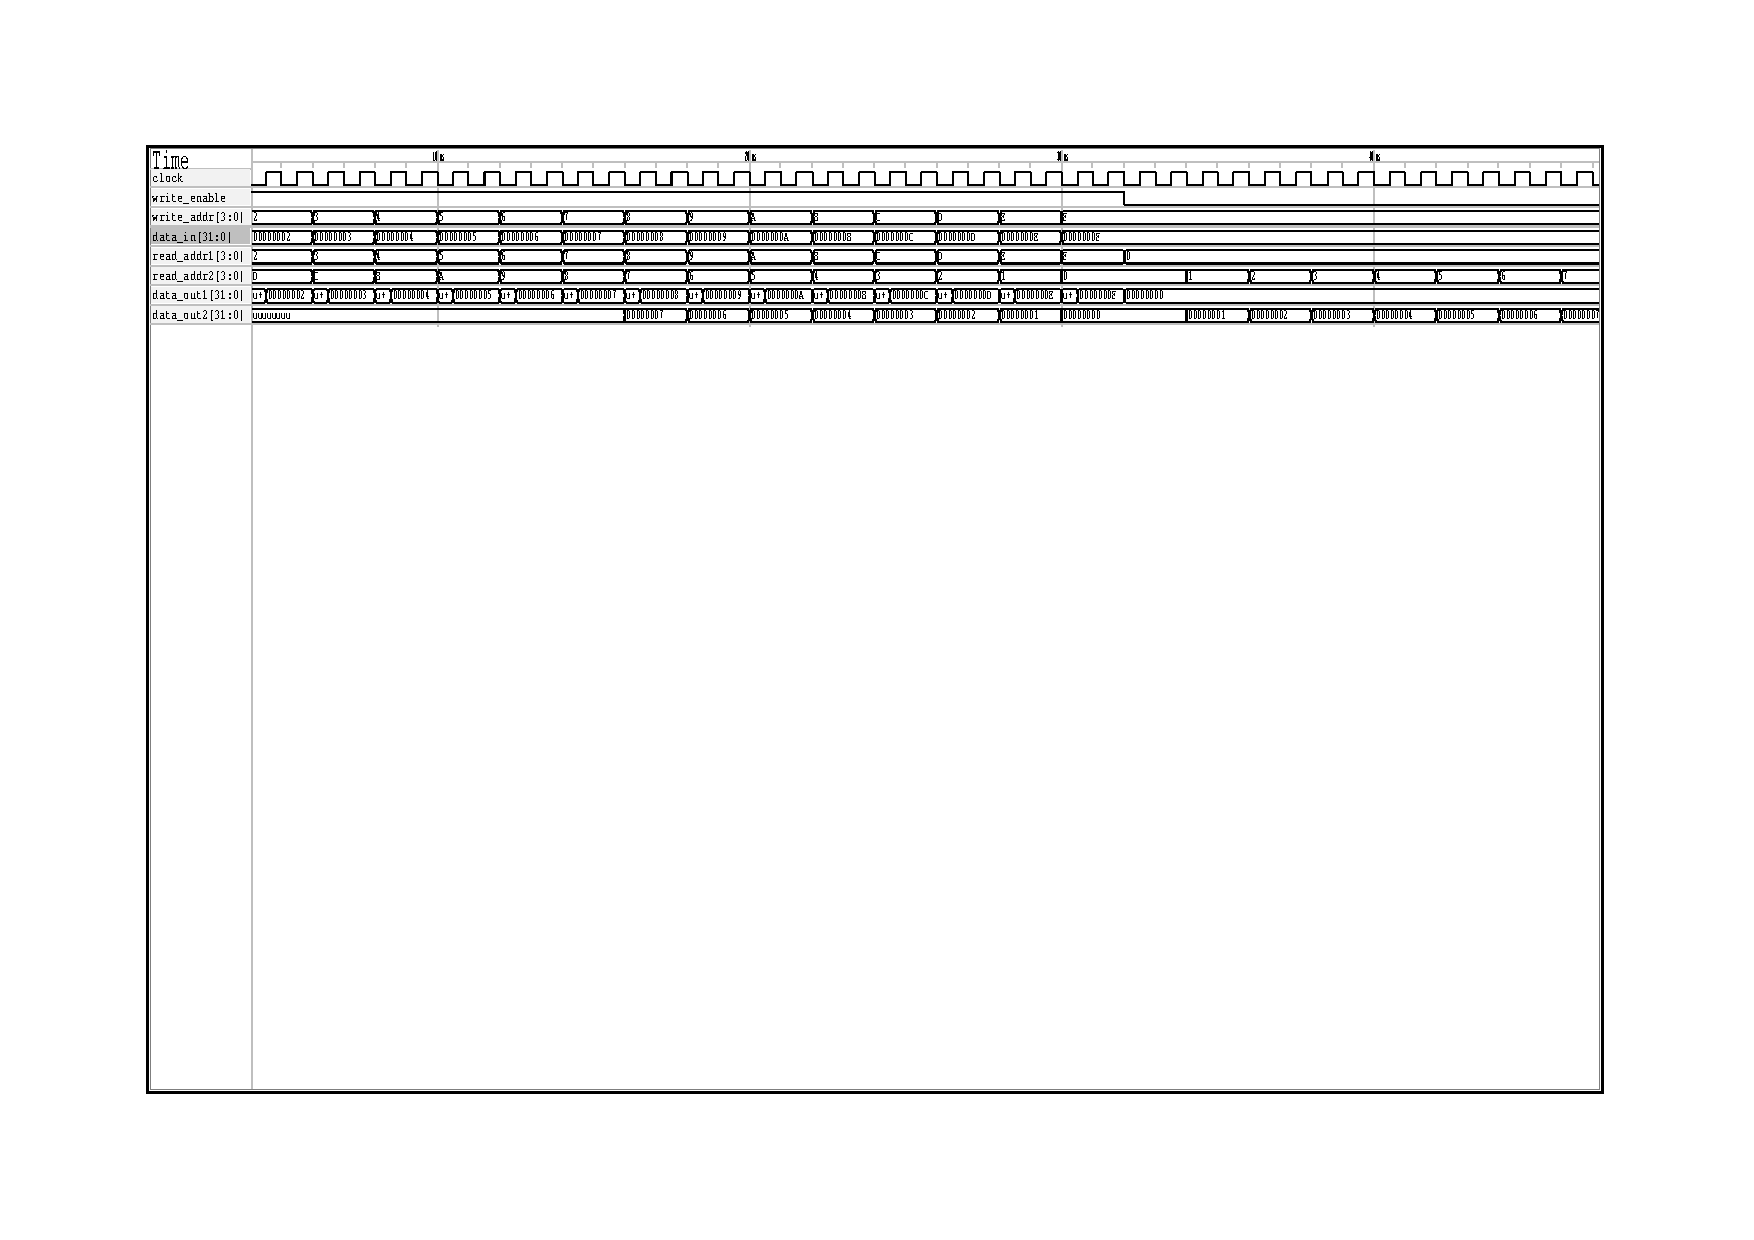
\includepdf[landscape=true, picturecommand*={\put (\LenToUnit{.05\paperwidth},20) {\tt{reg_file_tb.pdf}};}]{../output/reg_file_tb.pdf}
\end{document}
